% !Mode:: "TeX:UTF-8"
% 光信道建模:线性信道(小信号)与非线性(大信号)信道模型

\chapter{室内可见光通信系统灯组布局优化}\label{chap:led-layout}
\section{引言}
在可见光通信系统中,灯组必须兼具室内照明和数据通信两大功能,而室内可见光通信系统通常是由多个灯组组成的,因此对于灯组分布的优化就成为了一个重要的问题。
不同的灯组的分布,对应着不同的光照强度和不同的光接收功率分布。从文献[]中可以知道,合适的室内灯组分布,需要能够尽量使得光照强度和光接收功率均匀化。
同时,为了满足数据通信的基本要求,合适的灯组布局还需要尽可能地提高平均光接收功率强度,以满足高速的数据通信需求。
同时,在考虑LED灯组的安置问题的同时,由于系统使用的LED灯组通常是由多个LED灯组成的,因此还需要考虑灯组内的LED等应该如何组织这个问题。
在本章中,将会首先分析系统采用的可见光通信灯组的模型,并在此模型的基础上,提出了针对于光照强度和光接收功率这两个指标进行优化的灯组分布优化方案,
并给出了优化的仿真结果和光照强度分布和光接收功率分布曲线,以检验灯组布局优化的效果。

\section{可见光通信灯组模型}\label{sec:led-model}
\subsection{白光LED特性介绍}
LED是一种能够发光的半导体的电子元器件,其早期出现时只能发低光度的红光,后来在不断地研究中,出现了白光发光二极管,发光度也得到了很大的提升,从而使得白光二极管被应用于家用的照明中。
发光二极管只能够在一个方向导通,叫做正向偏置,当电流流过时,电子与空穴在其内重合而发出单色光,这叫电致发光效应[47]。
由于白色LED转化效率高,反应快,可靠性强,环保等特点,且其使用的成本已经大大低于目前的常用灯源,所以白光LED已经开始大范围地应用于家庭照明中。

LED的发展可以概括为由单一光向白光的转变,由低效率向高效率的转变。
在1961年,美国德州仪器公司的研究人员首次发现砷化镓等半导体合金会进行红外放射作用。
并于次年,有美国通用电气公司的研究人员开发出了可以被使用的可见光二极管。
在1993年,日本的中村修二利用镁掺入,发明了高亮度的蓝色发光二极管,并因此获得了2014年的诺贝尔物理学奖,以表彰其在白色环保能源方面的重要贡献。
在蓝色发光二极管被发明之后,白色发光二极管也随即问世,为室内的照明提供了基础。
但是当前的LED的发光强度仍然较低,在之后的20年中,为了制作出更加实用的LED灯,各大企业和研究机构不断投入资金,提高LED等的光照性能。
其中,日本的发光二极管厂商日亚化工和美国发光二极管厂商科锐不断地刷新LED的光效记录。在2012年4月,美国科瑞公司的LED光效已经能到达到254 lm/w。

常见的白光LED发光的方式按照发光二极管数量的不同可以分为单晶体和多晶体两种类型[48]。多晶体是指采用互补的LED发光二极管或者是将蓝红绿三种颜色的发光二极管组合在一起,混合之后产生白光。
这种方式发成的白光色域较宽,同时比其他方式的效率高,但同时生产成本也较高。另外一种正被大规模采用的LED生产方式就是采用单晶体方式,单晶体是指首先使用某一单元发出单一颜色波长较短的光,
比如蓝光或者是紫光,再使用磷光剂将短波长的光转化成长波长的白光。由于在转化过程中部分能量转化为热能,会造成能量的消耗,所以这种方式产生白光的发光二极管效率较低。

传统的照明,比如说荧光灯,白炽灯等,是装载有气体的玻璃管的形式,因此并不如被称为固态照明的发光二极管实用。
由于当增加二极管的光度时,二极管的效率也会下降,所以对于需要使用LED获得高亮度的情况,一般都是采用多个小的LED灯组成成为一个LED光源,而对于一些对光度要求低的场合,
单个的LED等也可以被直接使用来满足照明需求。

在1967年法国举行的第十三届国际计量大会上,``坎德拉'',``坎德拉/平方米'',``流明'',``勒克斯''被分别作为发光强度,光亮度,光通量和光照度的单位,作为照明领域最常用的几个量度。
其中光强度是指光源在指定方向的单位立体角内发出的光通量。绝对黑体在铂的凝固温度下,从5.305*10cm面积上辐射出来的光通量被定义为1lm。光亮度指发光表面在指定方向上的发光强度与垂直于指定方向的发光面积之比。
而光照度的定义为,被光均匀照射的物体,在1平方米面积上得到的光通量是1流明时,它的照度就是1勒克斯。

\subsection{室内LED灯组结构}
本章中将研究典型的室内光通信场景模型,并以此为基础进行灯组分布的优化。以一般的光通信应用场景,如办公室或者是会议室为例,本章设置了一个5*5*3的房间模型。
在该房间中安装有四个LED灯组,每个灯组被安放在距离地面2.5米的位置,房间中运动的用户的手持接收终端假定都处于1米的接收平面上,其灯组在室内的平面示意图如下图所示。

\begin{figure}[htbp]
    \centering
	\includegraphics[width=0.8\textwidth]{figures/chapter-3/LedLayout.eps}
	\caption{室内可见光通信灯组分布基本模型}
	\label{fig:led-layout-pic}
\end{figure}

对于发射端而言,为了提高LED灯组的照度和覆盖范围,每个LED灯组都包含有3600(60*60)个LED灯。
对于每一个LED而言,其发射半角是确定的,为70度,其中心的发光强度为0.73cd,中心的发光功率为20毫瓦。
对于用户接收器而言,其接收器探测表面积为1平方厘米,用户接收视场角为60度,光电转化效率为0.53A/W,
光滤波器的增益为1,其所有参数均列表显示如下。

\begin{table}[htbp]
    \caption{光通信灯组布局中使用的参数值}
    \label{tab:led-layout-param}
    \centering
    \begin{tabular}{llll}
        \toprule
        参数 & 取值 & 参数 & 取值\\
        \midrule
        房间长*宽*高     & 5*5*3($m^3$) & 接收视场角          & 60deg. \\
        接收平面高度     & 1m           & 一个灯组包含的LED数 & 60 \\
        LED中心发光强度  & 0.73lm       & 接收端检测面积      & $10^{-4}$ ($m^2$) \\
        LED中心发送功率  & 0.02w        & 光滤波器增益        & 1 \\
        发射机半功率角   & 73deg.       & 光接收器增益        & 3 \\
        光电转换效率     & 0.53         & 接收端折射系数      & 1.5 \\
        \bottomrule
    \end{tabular}
\end{table}

一般来说,在构建一个室内可见光通信系统时,在上述提及的参数后,还需要确定的变量就是灯组在安装平面的位置,以及组成LED灯组的各LED灯之间的间隔。
这两个参数值也将会直接影响到光照分布和光通信系统的通信质量,下文中也将以这两个变量作为优化的参数。

\subsection{灯组分布优化方案}\label{sec:led-layout-design}
为了保证房屋内的照明和高质量通信的要求,需要在上述灯组结构的基础上,对室内灯组的具体位置指标进行设计。首先,需要明确室内灯组布局优化的几个目标。
第一点,设计的灯组的布局应该能使得室内的光照分布和接收光功率分布要尽可能地均匀,从而使得用户在室内照明和数据通信上都可以获得良好的使用体验,
第二点,室内光通信的目标是实现高速短距离的数据通信,灯组的布局优化也应该以此为目标,通过对灯组的布局调整,在用户接收端获得较高的接收功率,
第三点,根据国际标准化组织的规定,办公室内合适的光照强度的范围为300-1800lm,此范围的光照强度会让人感到最为舒适,因此规定的室内光照强度范围必须是灯组布局设计的一个重要依据。
根据上文描述,假定每个LED灯组的发射功率都是一样的,灯组在室内组装时,可以通过优化灯组摆放在房间中的位置和灯组之间的间隔,满足室内照明和通信的需求。

根据上文的分析,灯组布局优化问题可以看作为通过设计几项参数使得设计的目标达到最优的这样一个问题,因此可以采用了一个最优化模型对灯组布局优化问题进行建模。在进行最优化灯组布局建模时,将系统优化的参数用一个向量x来进行表示:

\begin{equation}
    x=\left[d \quad i\right]^T
\end{equation}

其中$d$表示的是灯组距离房间中心点的水平方向上的距离,$i$表示的是灯组之间的距离,如下图所示。

\begin{figure}[htbp]
    \centering
	\includegraphics[width=0.8\textwidth]{figures/chapter-3/LedLayoutDI.eps}
	\caption{光通信室内灯组分布参数示意图}
	\label{fig:led-layout-d-i}
\end{figure}

上述需要考虑的目标问题也就成为模型需要考虑到多个优化目标,其中第一点的目标要求最大化模型的光照强度和光接收功率的均匀度,将该目标函数设为$f_{1}(x)$。
第二点的目标要求最大化模型的接收平面的平均光接收功率,将该目标函数设为$f_{2}(x)$,第三点,则可以成为最优化模型的接收条件。
由于第一点和第二点的目标函数是不能同时达到最优的,即系统不太可以在光照强度和光接收功率很均匀的情况下,获得最好的平均光接收功率,因此,本文的最优化模型也就变成了多目标优化的模型,如下式所示。

\begin{equation}
\begin{aligned}
    \max\quad & \left[f_{1}(x) \quad f_{2}(x)\right] \\
    \mbox{s.t.}\quad & 300\le minE_{or}(x) \le maxE_{or}(x) \le 1800 \\
           & 0 \le d \le 2   \\
           & 0 \le i \le 0.04 \\
           & d+\frac{n-1}{2}*i \le L
\end{aligned}
\end{equation}


其中,$E_{or}(x)$表示的是系统灯组参数为$x$的情况下的光照强度分布,$n$表示的是灯组中一排的LED数目值,根据前文中对灯组结构的描述,该值被设置为60,$L$为房间的宽度的一半。

对于上述的各目标函数,需要进行定量地分析。目标一中的均匀度可以分别使用灯组光照分布的方差和光接收功率分布的方差进行衡量,要求计算出的结果是越大越好,
系统的均匀度的目标取决于上述的这两个方差目标,假设灯组在某一灯组布局参数条件下的光照分布的方差为$\delta_{e}(x)$和光接收功率分布的方差为$\delta_{p}(x)$,那么就可以得到这两个方差组合成的在某一灯组布局参数条件下对均匀度目标函数:

\begin{equation}
    f_{1}(x)=-\delta_{e}(x)-\delta_{p}(x)
\end{equation}

另外,需要考虑的还有目标二中的目标函数,这里可以直接采用平均接收功率强度去衡量,同样,假设在某一灯组布局参数条件下的平均光接收功率为$\overline{P}_{or}(x)$,那么目标二的目标函数为

\begin{equation}
    f_{2}(x)=\overline{P}_{or}(x)
\end{equation}

因此要优化的目标函数则变为

\begin{equation}
    max \left[-\delta_{e}(x)-\delta_{p}(x)\quad \overline{P}_{or}(x) \right]
\end{equation}

对于该复杂的多目标优化问题,本文采用统一目标函数法将该问题转变为单一目标的最优化函数来进行简化,这里采用较简单的线性加权法来进行处理,线性加权组合法的基本思想就是在多目标最优化问题上,
将其各个分目标函数根据其数量级和在整体优化设计中的重要程度相应地给出一组加权因子,再进行线性组合,从而构成一个新的统一单目标函数。

同时,由于本模型中的两个目标函数都是具有单位的,因此不能被直接进行线性加权使用,因此,首先需要对均匀度和平均光接收功率这两个目标函数值进行归一化,本文中两个目标函数都按照如下的归一化方法进行

\begin{equation}
    \overline {f(x)}  = \frac{{f(x) - \min f(x)}}{{\max f(x) - \min f(x)}}
\end{equation}

归一化后的数据值都将变为0和1之间。

由于本文中的目标函数个数为2,因此,只需要假设一个参数因子$\alpha$,处理后得到的新的目标函数为

\begin{equation}
    \max f(x) = \alpha  \times \overline {{f_1}(x)}  + (1 - \alpha ) \times \overline {{f_2}(x)}
\end{equation}

其中,$\overline {{f_1}(x)}$和$\overline {{f_2}(x)}$分别表示归一化后的目标函数一和目标函数二。

于是,该优化问题就转变为一个多个约束条件下的单目标优化问题,同时对于$\alpha$的值,可以灵活地调节,在趋向于分布均匀的室内光强和光功率和趋向于更高平均接收功率的光强分布之前进行平衡,以获得所期待的光照强度和光功率分布结果。

\section{仿真实验及结果分析}\label{sec:led-layout-simulation-result}
上根据上述的理论分析,本文通过Matlab软件建立了室内可见光通信模型,并按照上述的最优化模型在约束范围内搜索使得目标函数达到最大的灯组最优分布结果。
在结果展示中,分别通过计算室内的光接收功率分布和光照强度分布来描述模型优化对室内照明和通信质量这两方面的影响。

根据上文中模型的描述,模型参数 决定的是系统在均匀度和光接收功率这两个目标上的分别的权重,所以我们可以通过改变 的值,来考察模型在不同的均匀度和接收功率需求下的灯组的最佳分布。

\subsection{偏重平均光接收功率的最佳灯组布局}
为了查看系统在高光接收功率需求下的优化结果,令模型中 取值为0.1,也就意味着在统一评价目标更加看重于平均光功率这一目标,此时,模型搜索出来的灯组放置结果为:$d = 1.2$,$i = 0.015$。

仿真得到的光功率分布图和光照强度分布图如下所示。

\begin{figure}[htbp]
    \centering
	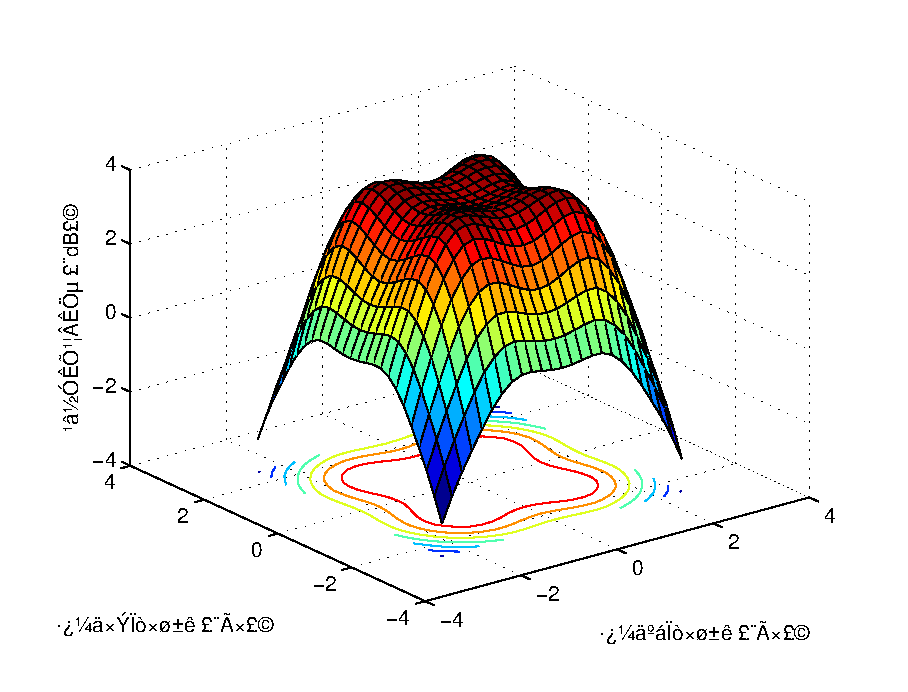
\includegraphics[width=0.7\textwidth]{figures/chapter-3/PowerFirstPower.eps}
	\caption{偏重平均光接收功率时的光接收功率分布}
	\label{fig:power_first_power}
\end{figure}

\begin{figure}[htbp]
    \centering
	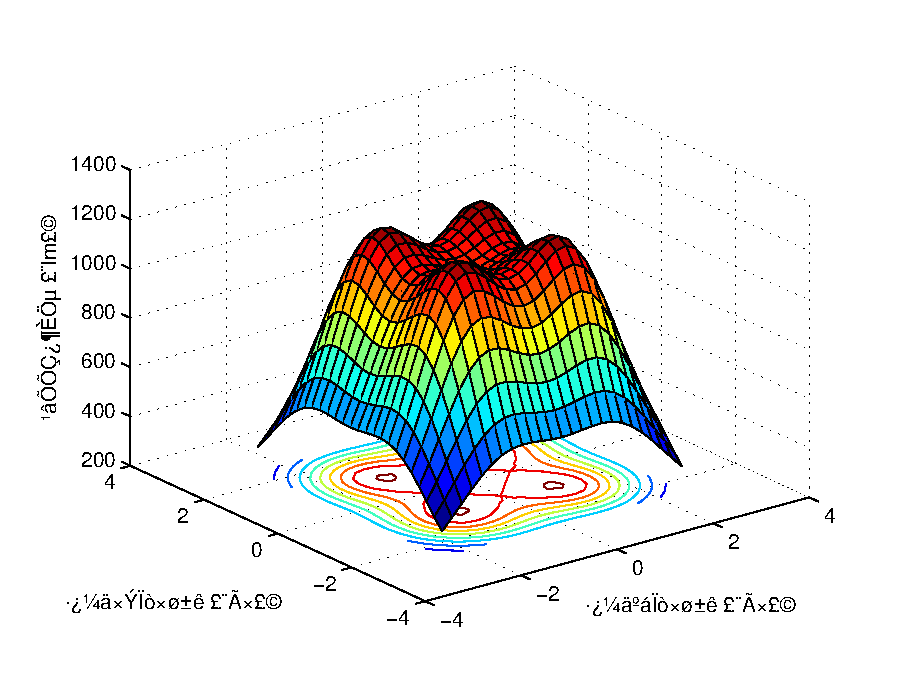
\includegraphics[width=0.7\textwidth]{figures/chapter-3/PowerFirstIllu.eps}
	\caption{偏重平均光接收功率时的光照强度分布}
	\label{fig:power_first_illu}
\end{figure}

从上图中可以看到,当对系统的光接收功率要求较高时,此时优化后的灯组将会被放置在更靠房屋中心的位置,且四个灯组的放置都较为集中,使用在房屋中心区域的光接收功率较高,
然后向外依次递减,此时,光功率最大值为3.9932dBm,最小值为-3.1157dBm,平均值为1.9982dBm。光照强度最大值为1213lm,最小值为301lm,平均值为857lm。

在这种灯组布局情况下,室内中心区域的光照强度较高,光接收功率值也较高,用户可以再室内中心区域获得很好的通信质量和照明效果,但是其对边缘区的覆盖不足,
会导致当用户运动到室内的边缘区域后,其光通信的质量会出现迅速的下降,照明效果也远差于中心区域。

\subsection{偏重整体均匀度的最佳灯组布局}
同时,为了研究系统在对整体均匀度要求较高时的灯组优化布局情况,我们可以将模型中的 设置为0.9,在计算系统评价函数时更加看重于光照强度和光功率的均匀度,同
样对设定的可行域进行搜索之后,通过仿真可以获得灯组的最优分布为$d = 1.7$,$i = 0.025$。

在该情况下得到的最优光功率分布和光照强度分布分别为

\begin{figure}[htbp]
    \centering
	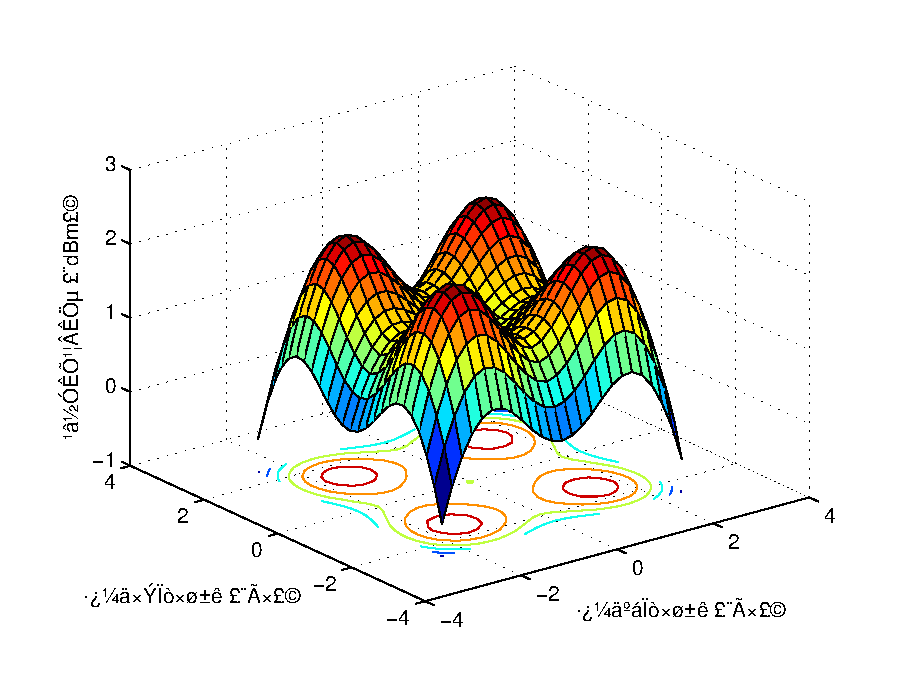
\includegraphics[width=0.7\textwidth]{figures/chapter-3/BalanceFirstPower.eps}
	\caption{偏重整体均匀度时的光接收功率分布}
	\label{fig:balance_first_power}
\end{figure}

\begin{figure}[htbp]
    \centering
	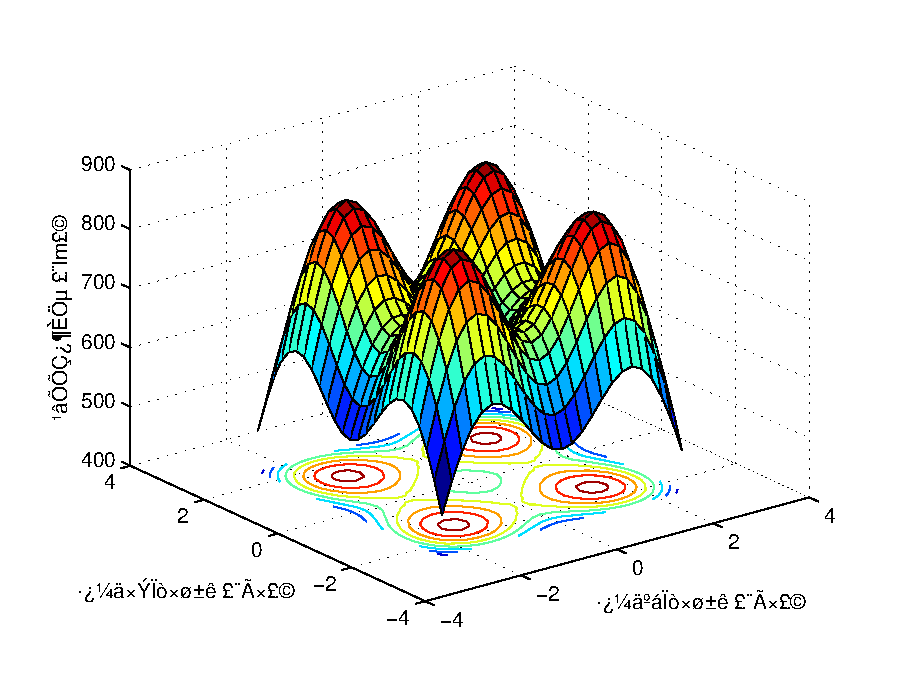
\includegraphics[width=0.7\textwidth]{figures/chapter-3/BalanceFirstIllu.eps}
	\caption{偏重整体均匀度时的光照强度分布}
	\label{fig:balance_first_illu}
\end{figure}

根据上图,当模型对系统的均匀度要求比较高时,灯组在室内的布局将会更加分散,同时灯组之间的距离也会相应地拉大,以保证系统指标的更可能的均匀化。仿真得到的光照强度和光接收功率值的变化范围也随之减小了。
此时,光功率最大值为2.2549dBm,最小值为-0.5681dBm,平均值为1.2765dBm。光照强度最大值为866lm,最小值为469lm,平均值为702lm。

在上述灯组布局下,可以看到灯组的分散放置使得室内光照和光通信的覆盖范围都得到了扩大,用户在除了墙角区域的其他区域都可以获得相对均匀地覆盖,
这样布局方式可以最大限度地扩大用户可进行可靠光通信的活动范围,也不易察觉到由于用户位置移动导致的通信质量的强烈变化。

\subsection{综合考量下的最佳灯组布局}
为了兼顾光接收功率和光照强度的均匀性和尽可能地扩大光功率强度,可以调节一个适中的 值来获得对两个指标综合考量下的最优分布。
在本文中,我们取$\alpha$的值为0.5,可以获得该情况下的最优分布为$d = 1.4$,$i = 0.02$。

此时的光功率分布和光照强度分布如下图所示

\begin{figure}[htbp]
    \centering
	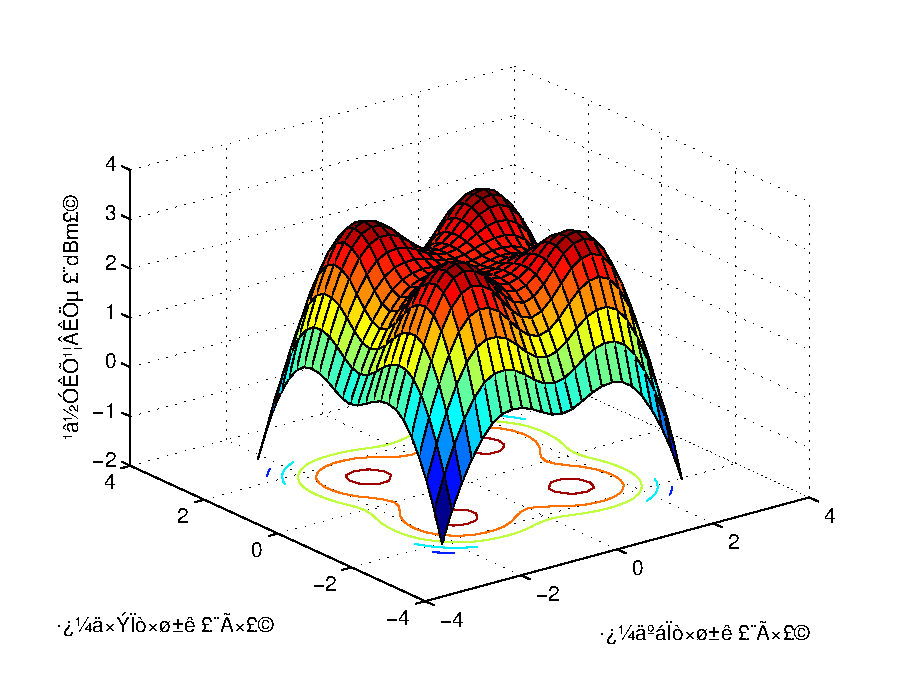
\includegraphics[width=0.7\textwidth]{figures/chapter-3/BestPower.eps}
	\caption{综合考量时的光接收功率分布}
	\label{fig:best_power}
\end{figure}

\begin{figure}[htbp]
    \centering
	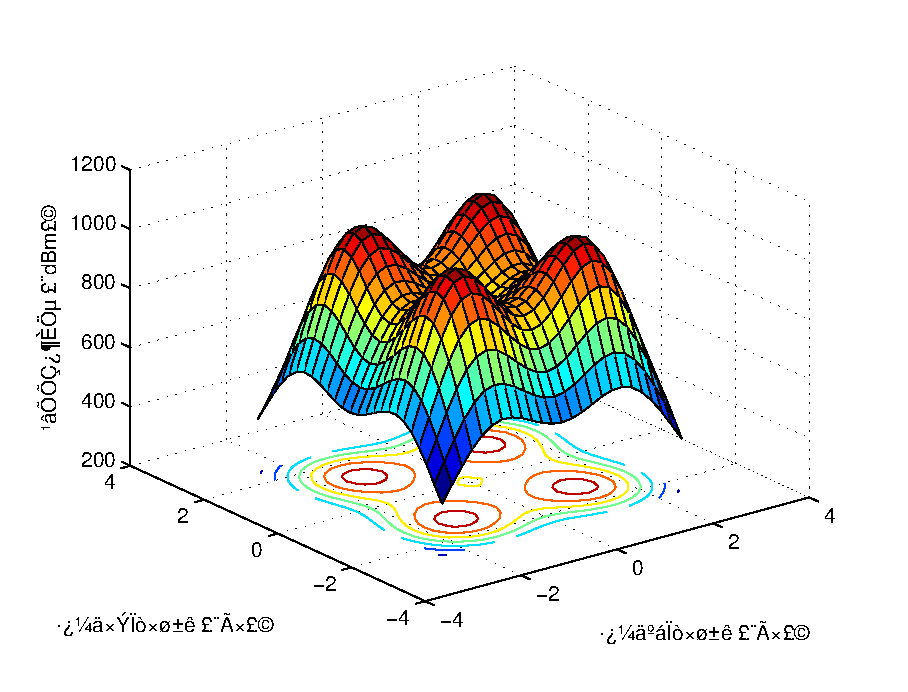
\includegraphics[width=0.7\textwidth]{figures/chapter-3/BestIllu.eps}
	\caption{综合考量时的光照强度分布}
	\label{fig:best_illu}
\end{figure}

从上图中,我们可以看到当系统要求兼顾指标的均匀度和光接收功率时,灯组的布局则可以看作为上述两种情况下的折中安置,不管是灯组距离室内中心点的距离还是灯组之间的间距,都处于一个比较平衡的值。
在该情况下得到的室内系统参数值为:光功率最大值为3.1840dBm,最小值为-1.7493dBm,平均值为1.7850dBm。光照强度最大值为1047lm,最小值为377lm,平均值为792lm。

在上述灯组布局下,可以看到灯组的分散放置使得室内光照和光通信的覆盖范围都得到了扩大,用户在除了墙角区域的其他区域都可以获得相对均匀地覆盖,
这样布局方式可以最大限度地扩大用户可进行可靠光通信的活动范围,也不易察觉到由于用户位置移动导致的通信质量的强烈变化。

在上述条件下的灯组布局,则是比较实用的灯组布局方式。可以看到这种布局方式,不仅可以保证室内的光照范围和光通信覆盖范围尽可能地广,
又可以保证在室内的大部分区域中的光接收功率较大,用户的高速通信需求可以得到保证。因此,这种综合考量下的布局方式可以在实际灯组的布局中获得应用。

\subsection{用户的接收视场角对最佳灯组布局结果的影响}
灯组的最优化布局结果不仅和当前的用户照明需求有关,还和用户的接收视场角有关系,这里可以研究用户的接收视场角对最佳灯组布局的影响。在仿真中,将模型公平性参数$\alpha$ 值设定为0.5,改变用户的接收视场角FOV的大小分别为40度和80度时,仿真得到的两种情况下最优化布局的光接收功率分布分别为

\begin{figure}[htbp]
    \centering
	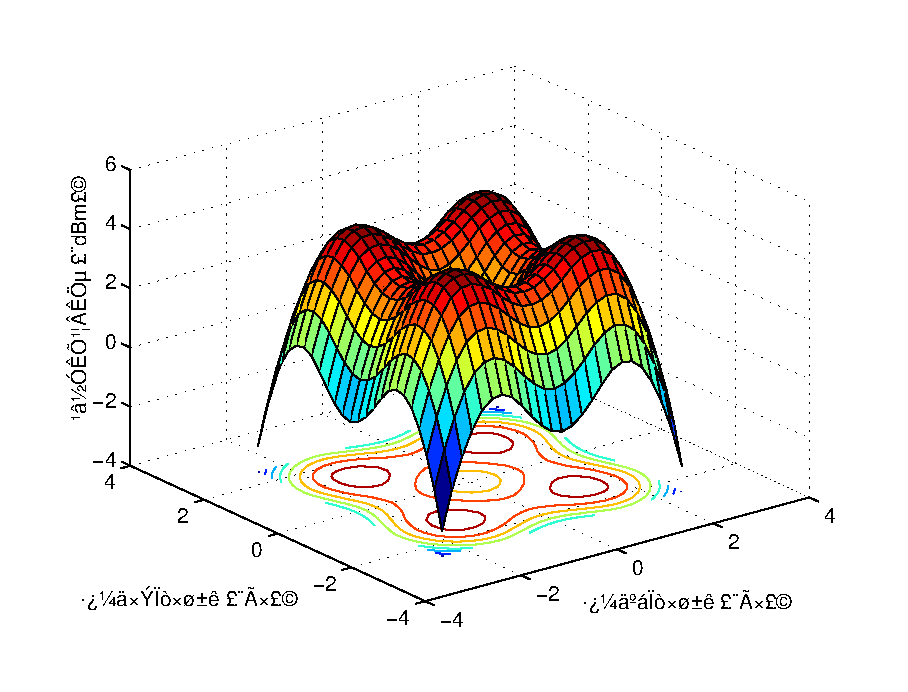
\includegraphics[width=0.7\textwidth]{figures/chapter-3/Fov40Power.eps}
	\caption{FOV值为40时的光接收功率分布}
	\label{fig:fov_40_power}
\end{figure}

\begin{figure}[htbp]
    \centering
	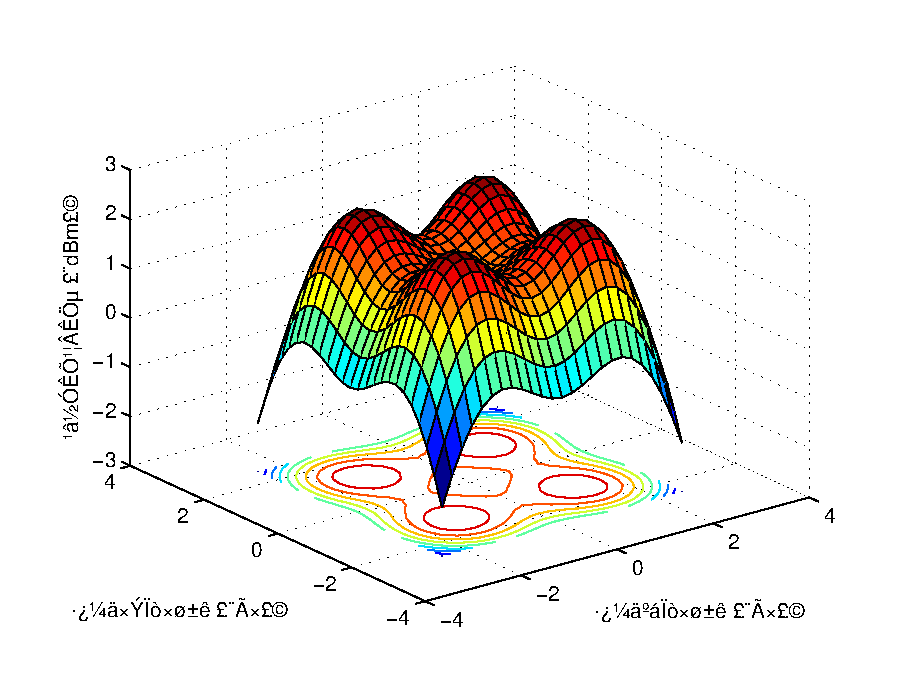
\includegraphics[width=0.7\textwidth]{figures/chapter-3/Fov80Power.eps}
	\caption{FOV值为80时的光接收功率分布}
	\label{fig:fov_80_power}
\end{figure}

上述直观地反映了FOV对光接收功率的影响,同时结合之前在FOV为60时仿真的数据,也可以通过下表中具体的数据来分析FOV的变化对灯组布局的影响。

\begin{table}[htbp]
    \caption{FOV的变化对灯组布局的影响}
    \label{tab:fov-vs-led-layout}
    \centering
    \begin{tabular}{lllllll}
        \toprule
        FOV值 & 最优d值 & 最优i值 & 光功率范围 & 平均光功率 & 光强范围 & 平均光强\\
        \midrule
        40度  & 1.3米  & 0.03米  & -3.1475 $\sim$ 4.4448dBm & 2.3580dBm & 350 $\sim$ 1017 & 800 \\
        60度  & 1.4米  & 0.02米  & -1.7493 $\sim$ 3.1840dBm & 1.7850dBm & 377 $\sim$ 1047 & 792 \\
        80度  & 1.4米  & 0.02米  & -2.0133 $\sim$ 2.4172dBm & 1.1109dBm & 377 $\sim$ 1047 & 792 \\
        \bottomrule
    \end{tabular}
\end{table}

从上表中可以看出,随着FOV角度的不断增加,其最优布局的平均光接收功率逐渐减小,而光接收功率范围的波动也在变小,表现在最终的灯组布局结果上,则是灯组距离房间中间的距离逐渐变大,
灯组之间的间隔也在随着FOV的增加而变小。而对于光照强度,在三种接收角度下,模型均能保证室内的光照强度处于一个较好的范围内,其均值都在800lm附近。这是因为当FOV的角度较小时,
用户只有在很小的范围内才能接收到灯组的信号,因此如果灯组之间的距离过远,那么在用户平面上的某些点时,用户收到的信号则会很微弱,某些点,如灯组的正下方,用户收到的信号又会很强,
所以灯组都被较为集中地放置,从而使得在FOV较小时牺牲了整体的均匀性,使得光接收功率上达到较优的状态。而随着FOV的逐渐增大,用户可接收到的灯组的范围也逐渐增加,这也就降低了之前让灯组集中布置的需求,
让灯组尽可能地分散开来布置,从而增加整体的均匀性,但是太多分散的灯组会降低整体的平均光接收功率,所以灯组之间的间隔就被逐渐地减小已作补偿,在均匀性和高光接收功率之间寻找一个平衡点。


\section{本章小结}
本章主要研究了室内可见光通信中灯组的最优化布局方式。首先,本章介绍了LED技术的发展历程和LED的发光原理,并介绍了室内照明中常见的度量单位。
接着,本章介绍了本文使用的室内光通信场景模型,并介绍了本文使用的LED灯的具体参数。对于如上提出的场景,本文根据室内照明和高速数据通信的需求,
提出了一种多目标的灯组布局最优化模型,充分考虑了室内照明和接收功率均匀度和光接收功率均值的影响。在模型的解决阶段,本章使用了线性加权法对模型进行了求解,
并通过调节模型中的参数因子,分别求解出对于高室内光照和光接收功率均匀度,高平均光接收功率,和综合考虑上述两种条件这三种情形下的灯组的最优分布,并分别给出了其相应的光接收功率分布和光照强度分布。
